% Этот шаблон документа разработан в 2017 году
% Владимиром Коротковым (kvamob@mail.ru) 
%  

\documentclass[a4paper,12pt]{article} % добавить leqno в [] для нумерации слева

%% Глобальные Параметры страницы
\usepackage[left=3cm,right=2cm,top=1cm,bottom=2cm,bindingoffset=0cm]{geometry}

%\usepackage{fp} 						% Вычисления с плавающей точкой
%\usepackage{siunitx}					% При использовании пакета fp все числа должны иметь decimal delimiter точку
%\sisetup{output-decimal-marker={,}}	% Числа выводятся с запятой в качестве разделителя разрядов: \num{3.2} выводит 3,2 

%%% Работа с русским языком
\usepackage{cmap}					% поиск в PDF
\usepackage{mathtext} 				% русские буквы в формулах
\usepackage[T2A]{fontenc}			% кодировка
\usepackage[utf8]{inputenc}			% кодировка исходного текста
\usepackage[english,russian]{babel}	% локализация и переносы

%%% 
%\usepackage{rotating}				% Поворот текста

%%% Дополнительная работа с математикой
\usepackage{amsmath,amsfonts,amssymb,amsthm,mathtools} % AMS
\usepackage{icomma} % "Умная" запятая: $0,2$ --- число, $0, 2$ --- перечисление
\usepackage{gensymb}	% Градусы
%% Номера формул
%\mathtoolsset{showonlyrefs=true} % Показывать номера только у тех формул, на которые есть \eqref{} в  тексте.

%% Шрифты
\usepackage{euscript}	 % Шрифт Евклид
\usepackage{mathrsfs} % Красивый матшрифт


%% Перенос знаков в формулах (по Львовскому)
% \newcommand*{\hm}[1]{#1\nobreak\discretionary{}
%	{\hbox{$\mathsurround=0pt #1$}}{}}

%%% Работа с картинками
\usepackage{graphicx}  % Для вставки рисунков
%\usepackage[export]{adjustbox}
\graphicspath{{images/}}  % папки с картинками
\setlength\fboxsep{3pt} % Отступ рамки \fbox{} от рисунка
\setlength\fboxrule{0.2pt} % Толщина линий рамки \fbox{}
\usepackage{wrapfig} % Обтекание рисунков и таблиц текстом


%%% Работа с таблицами
\usepackage{array,tabularx,tabulary,booktabs} % Дополнительная работа с таблицами
\usepackage{longtable}  % Длинные таблицы
\usepackage{multirow} % Слияние строк в таблице

%%% Подписи к рисункам и таблицам в русской типографской традиции
\usepackage{caption} 
\DeclareCaptionFormat{GOSTtable}{#2#1\\#3}
\DeclareCaptionLabelSeparator{fill}{\hfill}
\DeclareCaptionLabelSeparator{dot}{. }
\DeclareCaptionLabelFormat{fullparents}{\bothIfFirst{#1}{~}#2}
\captionsetup[table]{
	format=GOSTtable,
	font={footnotesize},
	labelformat=fullparents,
	labelsep=fill,
	labelfont=rm,
%	labelfont=it,
	textfont=bf,
	justification=centering,
	singlelinecheck=false
}
\captionsetup{font=small}
\captionsetup[figure]{
	labelsep=dot, 
%	textfont=it
}
% А можно и так
%\captionsetup{labelsep=period}


%%% Модификация команд, задающих разделы
% Не подавлять отступы у первого абзаца

\makeatletter   % Команда \makeatletter делает символ @ буквой, команда \makeatother возвращает всё на свои места.
% Разрешим отступ у первого абзаца
\renewcommand\section{\@startsection {section}{1}{\parindent}%
	{3.5ex \@plus 1ex \@minus .2ex}{2.3ex \@plus.2ex}%
	{\normalfont\hyphenpenalty=10000\Large\bfseries}}

\renewcommand\subsection{\@startsection {subsection}{1}{\parindent}%
	{3.5ex \@plus 1ex \@minus .2ex}{2.3ex \@plus.2ex}%
	{\normalfont\hyphenpenalty=10000\large\bfseries}}
\makeatother

% После номеров разделов \section ставить точки
\usepackage{secdot}			
% И после \subsection тоже ставить точки
\sectiondot{subsection}		


%%%%%%%%%%%%%%%%%%%%%%%%%%%%%%%%%%%%%%%%%%%%%%%%%%%%%%%%%%%%%%%%%%%%%%%%%%%%%%%%%%%%%%%%%%%%%%%%%%%%%%%%%
%%% PAYLOAD
%%%%%%%%%%%%%%%%%%%%%%%%%%%%%%%%%%%%%%%%%%%%%%%%%%%%%%%%%%%%%%%%%%%%%%%%%%%%%%%%%%%%%%%%%%%%%%%%%%%%%%%%%

%%% Заголовок
\author{ООО <<Гидросфера>>}\label{company}
\title{ОТЧЕТ ПО РЕЗУЛЬТАТАМ ПОИСКОВ ИСТОЧНИКОВ ПОДЗЕМНЫХ ВОД}
\date{\today}
%%%======================================================================================================
\newcommand{\txtExecutor}{ООО <<Гидросфера>>}	% Исполнитель
\newcommand{\txtYear}{2017}						% Год
\newcommand{\txtAddress}{--Address--}			% Адрес
\newcommand{\txtCadaster}{--Cadaster--} 		% Кадастровый номер


%%%%%%%%%%%%%%%%%%%%%%%%%%%%%%%%%%%%%%%%%%%%%%%%%%%%%%%%%%%%%%%%%%%%%%%%%%%%%%%%%%%%%%%%%%%%%%%%%%%%%%%%%

\begin{document} % конец преамбулы, начало документа

\setlength{\extrarowheight}{1mm} % Дополнительный интервал между строками таблиц

%% Титульная страница

\begin{titlepage}
	\begin{center}
		\textbf{\txtExecutor}
		\vspace{7.5cm}
		
		{\LARGE ОТЧЕТ ПО РЕЗУЛЬТАТАМ ПОИСКОВ}

		\bigskip

		{\LARGE ИСТОЧНИКОВ ПОДЗЕМНЫХ ВОД}
		
		\bigskip
		
		на участке по адресу:
				
		\underline{\txtAddress}
		
		\bigskip
		Кадастровый номер \txtCadaster
		
		\vfill
	
		\bigskip
		
	\end{center}

	\vfill
	
	\newlength{\ML}
	\settowidth{\ML}{«\underline{\hspace{0.7cm}}» \underline{\hspace{2cm}}}
	\hfill
	\begin{minipage}{1.0\textwidth}
		Директор ООО <<Гидросфера>> к.г.м.н.
		\underline{\hspace{\ML}} А.\,А.~Кашкаров\\
	\end{minipage}%
	
	\bigskip
	
	\vfill
	\begin{center}
		Екатеринбург, \txtYear
	\end{center}			

	\end{titlepage}

%%%%%%%%%%%%%%%%%%%%%%%%%%%%%%%%%%%%%%%%%%%%%%%%%%%%%%%%%%%%%%%%%%%%%%%%%%%%%%%%

\section*{Введение}

Изыскания источников подземных вод – важнейший этап в производстве комплексных работ по водоснабжению землепользователей за счет источников подземных вод, основанный изучении миграции подземных вод к местам их разгрузки.

Круговорот воды в природе чаще всего воспринимается как сток поверхностных вод к морям и океанам. Однако согласно статистическим сведениям, под землей хранится и перемещается на порядок больший объем воды, чем в реках и ручьях.

Теоретические и практические работы, выполненные автором настоящего заключения, убедительно показали, что участки земной коры, в которых наблюдается эффективная фильтрация подземной воды, имеют в поперечнике размер от 0,5 до 1,0 метра, по протяженности более 2 км, по глубине не превышает высоту изучаемого участка над уровнем моря. Такие участки наиболее перспективны для организации водозаборов. Именно они являются объектом изысканий, поскольку при минимальной глубине из них можно получить максимальный объем воды наиболее высокого качества. Качество воды определяется ее высокой обновляемостью в водоносных зонах, исключающую застойность, высокую минерализацию и жесткость.

Методы изысканий предполагают использование комплекса электроразведочных работ и оригинальный метод интерпретации, связанный с трансформацией геоэлектрических моделей грунтов в гидрогеологические и геомеханические модели.

\section{Цель изыскательских работ}
Целью выполненного комплекса изыскательских работ являются:
\begin{itemize}
	\item изучение геологического строения верхней части земной коры, литологии, стратиграфии процессов выветривания, техногенного изменения тектоники и т.д.
	\item инженерно-геологического строения верхней части земной коры с точки зрения фильтрационных возможностей грунтов, обеспечивающих перенос подземных вод к местам их разгрузки.
\end{itemize}


\section{Объёмы и виды изыскательских работ}
Для расшифровки геологической и инженерно-геологической ситуации на территории изучаемого участка землепользования выполнен следующий объем работ, приведенный в табл. {\ref{t:volumes}}.

\begin{table}\footnotesize
\caption{Объемы и виды выполненных работ}
\label{t:volumes}
\centering
\begin{tabulary}{\textwidth}{|C|L|L|L|L|}
	\hline 
	№№ п/п & Наименование работ & Ед. изм. & Объём & Решаемые задачи \\ 
	\hline 
	1. & Архивные и фондовые работы & печ. стр. & 200 & Оценка состояния свойств и геологии района работ \\ 
	\hline 
	2. & Рекогносцировочные работы & км & 4,0 & Оценка рельефа местности, описание обнажений  и выходов подземных и поверхностных вод \\ 
	\hline 
	3. & Геофизические работы методами электроразведки & точка & 30,0 & Оценка строения земной коры на глубину и по площади \\ 
	\hline 
	4. & Камеральные работы & \% от полевых & 30,0 & Описание и обработка материалов изысканий. Составление заключения \\ 
	\hline 
\end{tabulary} 
\end{table}

\section{Методика работ}

\subsection{Архивные и фондовые работы}
Архивные и фондовые работы выполняются квалифицированными инженерными работниками геологической специализации и связаны с анализом результатов комплекса геологических и инженерно-геологических работ прошлых лет.

На основании комплекса архивных и фондовых работ при анализе отчетного опубликованного и картографического материала дается характеристика геологии района и участка работ, состава и состояния грунтов по их устойчивости и перспектив водоносности, рельефа местности.

При грамотном выполнении архивных и фондовых работ дают наиболее точные рекомендации по технологии изыскательских и буровых работ и прогноз объемов, дебита проектируемых скважин и их конструкции.

\subsection{Рекогносцировочные работы}
Рекогносцировочные работы выполняют на изучаемой местности путем ее осмотра квалифицированным горным инженером – геологом методом маршрутных съемок по профилям, ориентированным вкрест выделенных геоморфологических структур или геологических неоднородностей.

При рекогносцировочных работах выполняют описание геоморфологии местности, обнажений, выходов подземных и поверхностных вод.

\subsection{Геофизические работы}
Если при изысканиях не применяют вскрышные работы, то геофизические изыскательские мероприятия являются основными методическими приемами инженерно-геологического и гидрогеологического исследования участка работ.

При изысканиях, связанных с оценкой инженерно-геологических и гидрогеологических параметров горных пород и массивов, связанных с оценкой устойчивости оснований фундаментов инженерных сооружений и оценкой перспективности участка для решения задач водоснабжения за счет источников подземных вод используют электроразведочные методы в глубинном и площадном вариантах.

Чаще всего используют три наиболее эффективных метода:  ВЭЗ (вертикальное электрическое зондирование), МСГ (метод срединных градиентов), ЕП (метод естественного поля).

Методом вертикального электрического зондирования изучается разрез грунтов на глубину и оцениваются геомеханические и фильтрационные параметры грунтов на разных глубинах.

Методом срединных градиентов изучается геологическое, гидрогеологическое и инженерно-геологическое строение земной коры по площади.

Методом естественного поля изучается гидрогеологическое строение земной коры в плане выявления зон, активно фильтрующих воду.

\section{Результаты работ}
\subsection{Результаты архивных и фондовых работ}
Участок работ расположен по адресу: \txtAddress.

В инженерно-геологическом отношении район работ относится к Урало - Тобольскому инженерно -  геологическому региону, расположенному в пределах средней и юго - восточной погруженной части Восточного склона Урала. С запада он граничит с Восточно - Уральским и Центрально - Уральским регионами, а также с Магнитогорским регионом, отделяясь от перечисленных регионов Восточным глубоким разломом. Восточная граница соответствует границе мезозойского чехла Западно - Сибирской плиты.

Регион протягивается по меридиану на 1000км от Верхотурья до Мугоджарских гор и Приуралья, включая Свердловскую, Челябинскую, Оренбургскую области Российской Федерации и Кустанайскую и Актюбинскую области Казахстана. В северной части ширина региона 80-120 км, в южной – 180-200 км.

\begin{figure}[h]
	\fbox{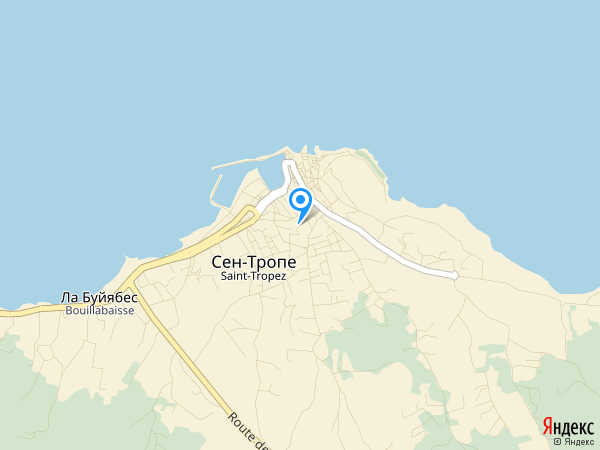
\includegraphics[width=\textwidth]{map}}
	%		\fbox{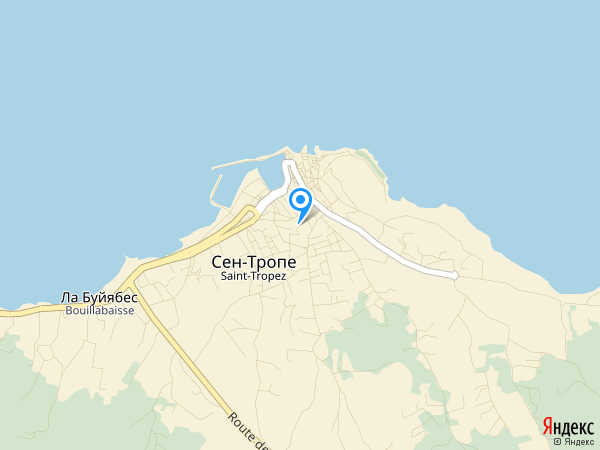
\includegraphics[width=650px]{map.png}}
	\caption{Обзорная карта района работ}
\end{figure}

Регион расположен на восточном склоне Урала в полосе Зауральского пенеплена, представляющего собой приподнятое холмистое плато, полого наклоненное к Западно-Сибирской равнине. Абсолютные отметки поверхности на Среднем Урале колеблются в пределах 260-380 м, на Южном Урале – 420-500 м. Междуречья ровные, участками всхолмленные. Долины рек широкие, хорошо разработанные с вогнутыми террасированными склонами. Относительные врезы долин составляют 30-40 м в западной и до 60-70 м в восточной части.

Речная сеть хорошо развита  и многоводна на севере, на юге мелководна и летом частично пересыхает. Модуль стока колеблется от 7-8 л/с на севере до 1 л/с на юге. Все крупные реки региона – Тагил, Нейва, Пышма, Исеть, Миасс,Уй, Тогузак принадлежат к бассейну р. Тобол.

В пределах региона расположено большое количество озёр, особенно на севере Челябинской области, где они нередко вытянуты в цепочки субмеридионального направления и приурочены к зонам тектонических нарушений. Наиболее крупные озёра: Аятское, Бол, Куям, Увильды. Южнее широты 56\degree отмечены солёные озёра, а на востоке Оренбургской области – горько-солёные и пресные бессточные неглубокие озёра (Шалкар-Ега-Кара и др.). 

Климат изменяется в направлении с севера на юг и с запада на восток, с учетом вертикальной зональности. Он относится к континентальному, с суровой и долгой зимой и жарким летом. Количество осадков уменьшается с севера на юг от 400-500 мм до 300 мм, теплый период выпадает 70\% осадков. Среднегодовая температура от 0\degree до +2\degreeС, абсолютный минимум -44\degreeС -- 52\degreeС, абсолютный максимум  от +36\degreeС до +42\degreeС. Мощность снегового покрова от 15 см до 100 см. Средняя глубина промерзания 150-220 см.

Глубина залегания уровня подземных вод изменяется от 10 м до выхода на поверхность. Воды безнапорные, местами слабо напорные.

По химическому составу подземные воды гидрокарбонатные кальциево-натриевые слабо минерализованные (0,1 -- 0,3 г/л).

Водообильность пород в целом незначительная и характеризуется фоновыми дебитами скважин 0,3 -- 0,5 л/с, достигая 2 -- 3 л/с и более в линейных водообильных зонах, связанных с тектоническими разломами и литологическими контактами.

\begin{figure}[h]
	\fbox{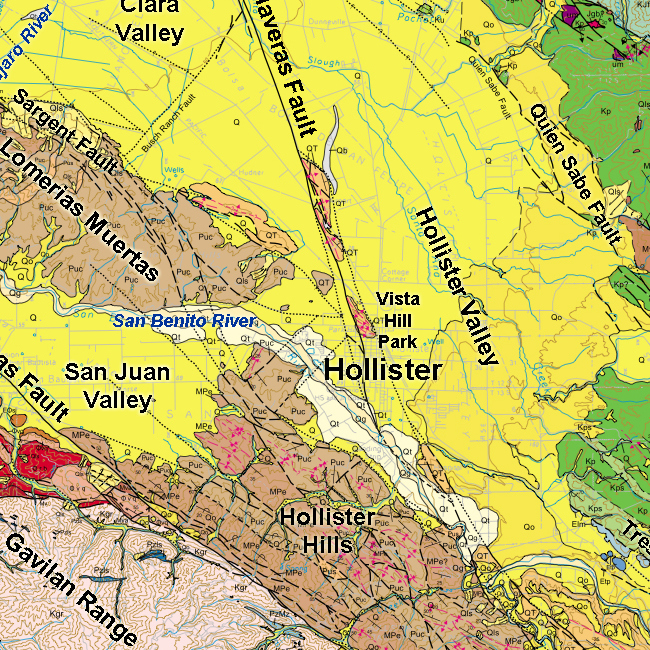
\includegraphics[width=\textwidth]{geomap}}
	%		\fbox{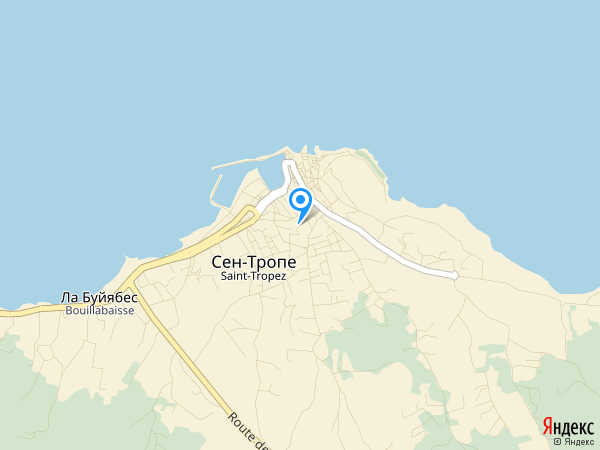
\includegraphics[width=650px]{map.png}}
	\caption{Геологическая карта района работ}
\end{figure}

\textbf{В геологическом  отношении} площадка  расположена  \textit{в зоне развития зеленых сланцев и рассланцованных эффузивов}. Скальные породы в верхней зоне сильно выветрелые, разбиты трещинами и  часто оталькованы. 

Элювиальная зона представлена щебенистыми грунтами с глинистым заполнителем до 10-15\%. Щебенистые грунты в коренном залегании напоминают подобие сплошной сухой кладки, постепенно переходящими в трещиноватую скалу. При бурении естественное сложение грунта нарушается, и извлекаемый керн представляется в виде малопрочных обломков.

С поверхности коренные породы перекрыты аллювиально-делювиальными образованиями - суглинками и глинами с включением щебня до 15\%.

\begin{figure}[!h]
	\centering
	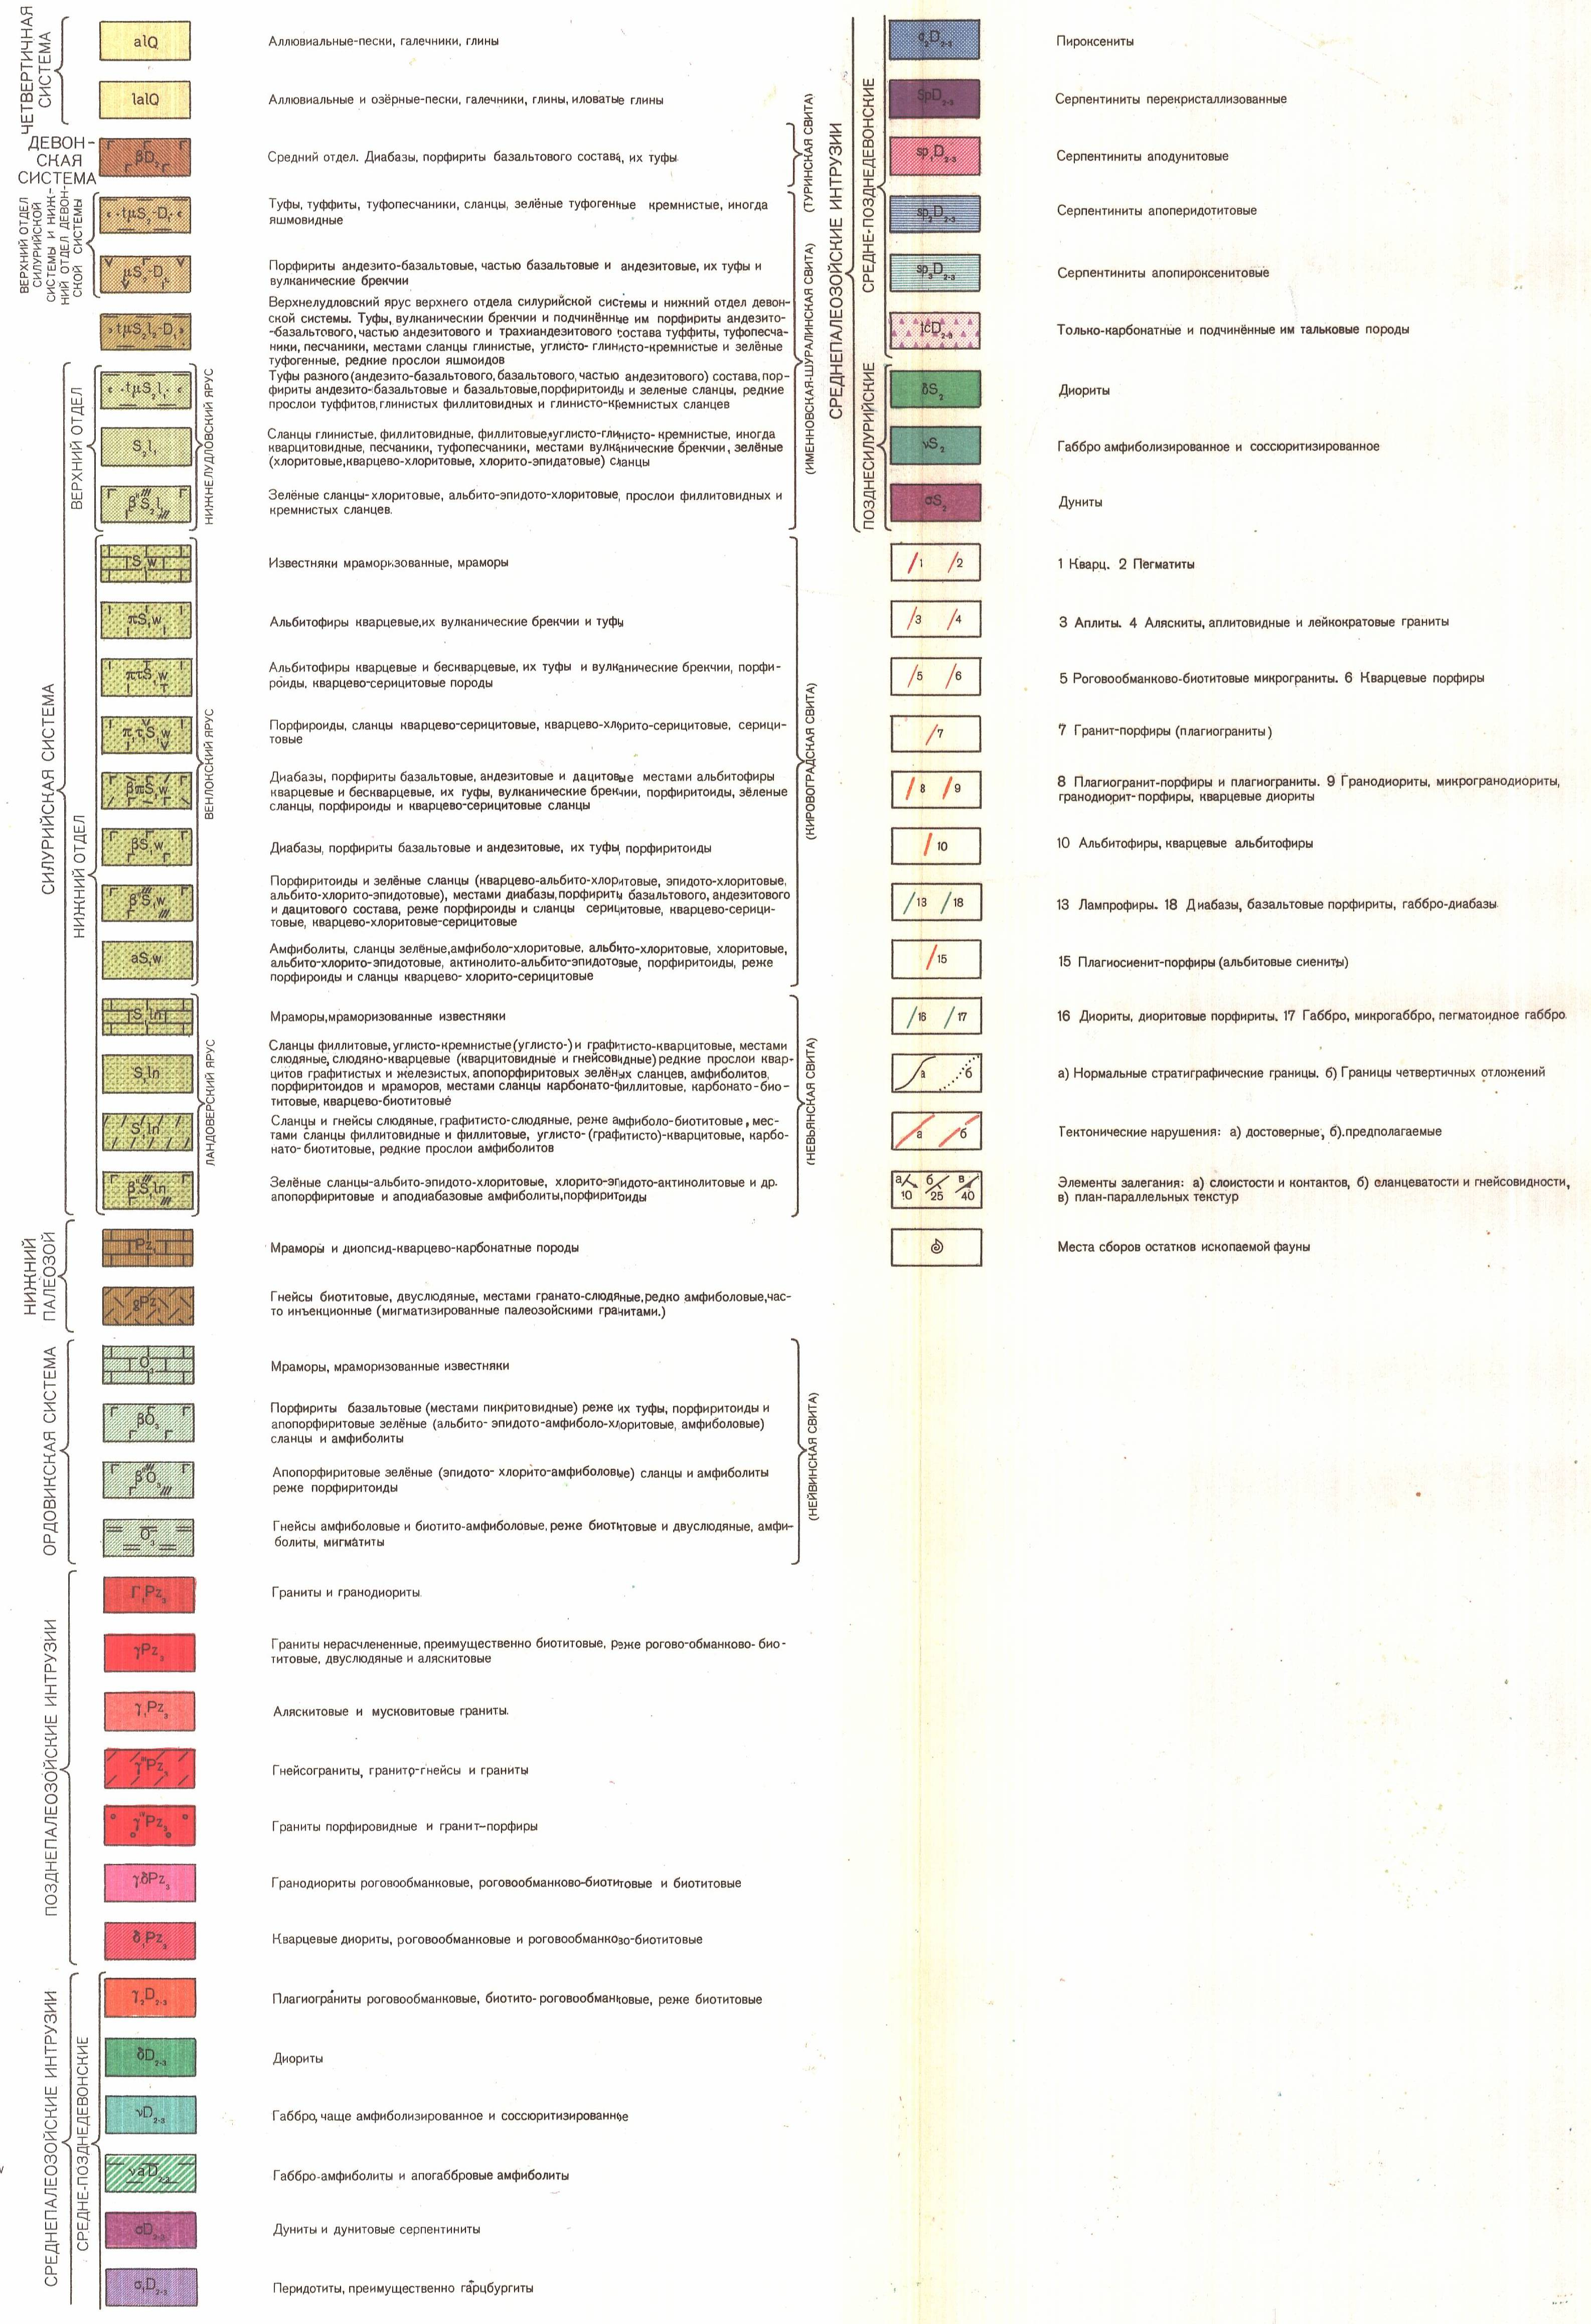
\includegraphics[height=0.95\textheight]{Legend-o-41-25}
	\caption[Условные обозначения]{Условные обозначения к геологической карте}
	\label{img:legend}
\end{figure}

\subsection{Результаты рекогносцировочных работ}
Рекогносцировочные работы, выполненные методом маршрутной съемки в районе площадки проектируемого строительства, позволили получить следующие результаты:

Участок работ сложен метаморфизованными сланцами, с включениями оталькованных участков. Верхняя часть разреза сложена слабопроницаемыми грунтами, поэтому существует реальная угроза подтопления зданий и сооружений и заболачивания участка. На участке имеются выходы подземных выработок.

\subsection{Геофизические работы}
Геофизические работы, выполненные методами электроразведки в вариантах ВЭЗ, МСГ, ЕП, позволили получить следующие результаты:
\begin{enumerate}
\item  В геоэлектрическом отношении участок работ является неоднородным. Удельные электрические сопротивления $\rho$ меняются от 50  до 300 Омм.
\item Колебания удельного электрического сопротивления грунтов связаны с неоднородностями геологического строения изучаемого разреза, вызванными процессами выветривания, тектоническими процессами.  
\item Метаморфические сланцы  имеют удельное электрическое сопротивление от 20 до 300 Омм, трещиноватые сланцы - от 50 до 100 Омм, кора выветривания и суглинки - 50 Омм, почвенно-растительный  $Q_{IV}$ - 10 Омм.
\item Выявлены взаимно пересекающиеся серии зон разгрузки подземных вод шириной 0,5 - 1,0 м, и длиной 1  км.
\item В выявленных зонах происходит интенсивная фильтрация подземных вод по контакту.
\end{enumerate}

\subsection{Камеральные работы}
На основе выполненных камеральных работ установлено:
\begin{itemize}
\item В пределах перспективного участка выделена серия водоносных зон сосредоточенной разгрузки подземных вод.
\item Наличие трещиноватых зон на глубине от 45 до 70 м в месте сосредоточенной разгрузки подземных вод.
\item Мощность выявленных водоносных зоны 0,6 м, простирание – до 1,5 – 2,0  км.
\item Положение выявленных зон показано на рис. 3
\item Место заложения скважины водоснабжения рекомендуется выбирать \textbf{в пределах узлов пересечения выявленных водоносных зон}.
\end{itemize}

\section{Рекомендации}
\begin{itemize}
\item Для обеспечения требуемых потребностей в воде рекомендуется проходка скважины водоснабжения в пределах узлов пересечения выявленных водоносных зон сосредоточенной разгрузки подземных вод. Ориентировочная глубина скважины в этом случае составит 40 – 45 м. Если расположить скважину вне пределов этих узлов, ее глубина составит не менее 70 м.
\item Положение скважины будет помечено на местности репером.
\item Обсадку трубами беcщелевой перфорации целесообразно выполнить  до коренных грунтов на глубину до 30  м от поверхности земли.
\item Во избежание попадания верховодки целесообразно применять обсадку трубами до глубины 5 - 10 м. 
\item Крайне не рекомендуется устройство заглублений вокруг устья скважины, для отвода воды из скважины необходимо использовать \textbf{водопровод  незаглубленного типа}, так как водопроводная траншея по сути является дренажной канавой, собирающей в себя поверхностные воды и «верховодку» далеко не лучшего качества, которые к тому же вымывают песок из суглинков, далее эти загрязненные воды с песком по затрубному пространству поступают в скважину, вызывая загрязнение и запесочивание скважины.
\end{itemize}


\end{document} % конец документа

